\documentclass[10pt,landscape,a4paper]{article}
\usepackage{multicol}
\usepackage[landscape]{geometry}
\usepackage{hyperref}
\usepackage[utf8]{inputenc}
\usepackage{minted}
\usepackage{graphicx}
\usepackage[binary-units]{siunitx}
\usepackage[usenames]{xcolor}
\usepackage{ulem}
\usepackage[english]{babel}
\usepackage{blindtext}
\usepackage{fontspec}
\setmainfont{Arial}
\setlength{\tabcolsep}{0.5em}
\geometry{top=0.5cm,left=0.5cm,right=0.5cm,bottom=0.5cm}
\usepackage{graphicx}
\graphicspath{ {./Bilder/} }

% Turn off header and footer
\pagestyle{empty}
 
% Redefine section commands to use less space
\makeatletter
\renewcommand{\section}{\@startsection{section}{1}{0mm}%
                                {-1ex plus -.5ex minus -.2ex}%
                                {0.5ex plus .2ex}%x
                                {\normalfont\large\bfseries}}
\renewcommand{\subsection}{\@startsection{subsection}{2}{0mm}%
                                {-1explus -.5ex minus -.2ex}%
                                {0.5ex plus .2ex}%
                                {\normalfont\small\bfseries}}
\renewcommand{\subsubsection}{\@startsection{subsubsection}{3}{0mm}%
                                {-1ex plus -.5ex minus -.2ex}%
                                {1ex plus .2ex}%
                                {\normalfont\footnotesize\bfseries}}
\makeatother

\setcounter{secnumdepth}{0}

\setlength{\parindent}{0pt}
\setlength{\parskip}{0pt plus 0.5ex}

\usepackage{enumitem}
\setlist{nosep}

%Define Colors
\definecolor{reg1}{HTML}{D6B656}
\definecolor{reg2}{HTML}{6C8EBF}
\definecolor{reg3}{HTML}{82B366}

\definecolor{green}{HTML}{4f9c45}
\definecolor{blue}{HTML}{0000ff}
\definecolor{red}{HTML}{ff0000}

%C-Code inline
\newcommand{\prgc}[1]{\mintinline{C}{#1}}

% -----------------------------------------------------------------------

\begin{document}

\definecolor{bluekeywords}{rgb}{0,0,1}
\definecolor{greencomments}{rgb}{0,0.5,0}
\definecolor{redstrings}{rgb}{0.64,0.08,0.08}
\definecolor{xmlcomments}{rgb}{0.5,0.5,0.5}
\definecolor{types}{rgb}{0.17,0.57,0.68}

\newcommand{\java}[1]{\mintinline{java}{#1}}
\newcommand{\xml}[1]{\mintinline{xml}{#1}}
\newcommand{\csharp}[1]{\mintinline{xml}{#1}}

\footnotesize
\begin{multicols*}{3}
\section{WPF- / .NET-Einführung}
.NET Framework: Single Plattform Impl. von .NET für Windows.

.NET Core: Cross Plattform, Open Source mit Fokus auf Desktop. 

Mono: Cross Plattform, Open Source Implementierung von .NET auf Mobile

NuGet ist der Paket Manager in .NET. Pakete sind ZIP-Archive (.nupkg). Pakete werden von öffentlichen oder privaten Hosts heruntergeladen. 

\section{WPF}
WPF läuft unter .NET Framework und .NET Core\\
Open Source\\
Nachfolger von Windows Forms\\
Trotz .NET Core: nur auf Windows ausführbar

Device Independent Pixels (DIP)\\
1 UI Pixel = 1/96 Zoll (in WPF)

\subsection{Hello World}
App.xaml -> Markup der Startup-Klasse\\
App.xaml.cs -> Code-Behind der Startup-Klasse\\
MainWindow.xaml -> Markup des Hauptfensters\\
MainWindow.xaml.cs -> Code-Behind des Hauptfensters\\
AssemblyInfo.cs -> Projektspezifische Meta-Daten

\begin{minted}{XML}
<Application x:Class="HelloWPF.App"
    xmlns="http://schemas.microsoft.com/
    winfx/2006/xaml/presentation"
    xmlns:x="http://schemas.microsoft.com/winfx/2006/xaml"
    xmlns:local="clr-namespace:HelloWPF"
    StartupUri="MainWindow.xaml">
    <Application.Resources> </Application.Resources>
</Application>

<Window x:Class="HelloWPF.MainWindow"
xmlns="http://schemas.microsoft.com/winfx/2006/xaml/presentation"
xmlns:x="http://schemas.microsoft.com/winfx/2006/xaml"
xmlns:d="http://schemas.microsoft.com/expression/blend/2008"
xmlns:mc="http://schemas.openxmlformats.org/
markup-compatibility/2006"
xmlns:local="clr-namespace:HelloWPF"
mc:Ignorable="d"
Title="Hello WPF" Height="350" Width="525">
    <Grid>
        <Label x:Name="HelloWorldLabel"
        Content="Hello WPF!"
        HorizontalAlignment="Center"
        VerticalAlignment="Center" />
    </Grid>
</Window>
\end{minted}
\begin{minted}{csharp}
namespace HelloWPF {
    using System.Windows;
    public partial class App : Application{ }
}

namespace HelloWPF {   
    using System.Windows;
    public partial class MainWindow : Window {
        public MainWindow() {
            InitializeComponent();
        }
}}
\end{minted}
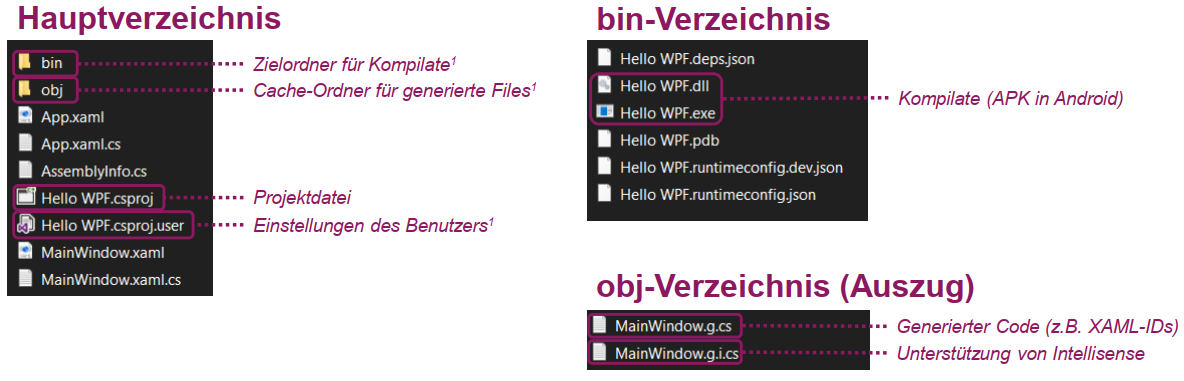
\includegraphics[scale=0.3]{images/generatedCode.PNG}
\subsubsection{Deployment}
\textbf{Framework-Dependent Executable (FDE)}:\\
• .NET Core muss manuell installiert werden\\
• Erzeugt sehr kleines Binary\\
\textbf{Self-Contained Deployment (SCD)}:\\
• .NET Core wird in Binary integriert\\
• Erzeugt grosses Binary (150 MB für Hello World)\\
• Ziel-Architektur muss beim Build gewählt werden

\section{XAML}
(Extensible Application Markup Language)\\
• XML-basiert\\
• Hierarchisch strukturiert (Baum)\\
• Trennung von Layout und Code\\
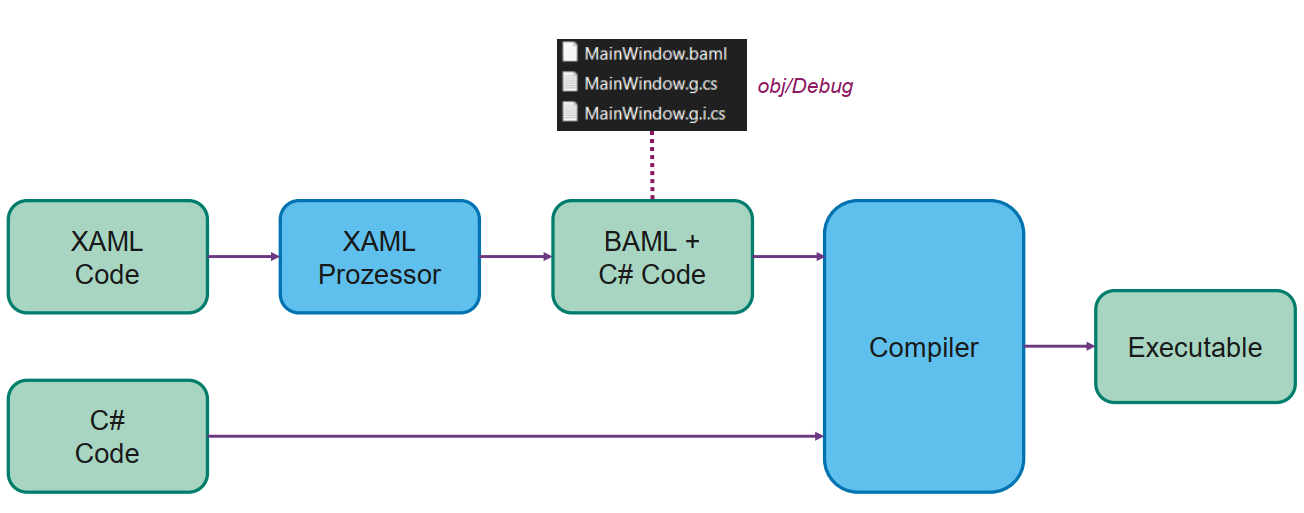
\includegraphics[scale=0.25]{images/Kompilation.PNG}
\textbf{Vorteile von XAML:}\\
• Oft leichtgewichtiger\\
• Oft kürzer und besser lesbar\\
• Grafischer Designer inklusive Vorschau\\
• Layout durch spezifische Tools erstellbar

\subsection{Beispiel Code im Codebehind}
\begin{minted}{csharp}
var button = new Button {
    Content = "OK", Height = 20,
    Width = 60, Margin = new Thickness(5)
};
var stackPanel = new StackPanel();
stackPanel.Children.Add(textBlock);
stackPanel.Children.Add(button);
this.Content = stackPanel;
\end{minted}
\section{Visual Tree}
Visual Tree (grün + blau)\\
• Vollständiger, gezeichneter Baum\\
• Enthält Elemente, die wir nicht selber definieren\\
Logical Tree (grün)\\
• Vereinfachung des vollen Baums\\
• Umfasst die durch uns definierten XAML-Elemente\\
\subsection{Namespaces}
\textbf{Mit xmlns werden XML-Namespaces definiert}\\
• Ohne Doppelpunkt: Standard-Namespace → Elemente können ohne Präfix verwendet werden\\
• Mit Doppelpunkt: Benannter Namespace → Elemente können nur mit Präfix verwendet werden\\
\textbf{Übliche Namespaces in WPF}\\
• Der Standard-Namespace wird auf die WPF Control Library gesetzt\\
• \textbf{x} für XAML-spezifische Elemente\\
• \textbf{d} für Elemente des visuellen Designers\\
• \textbf{mc} für Elemente der «Markup Kompatibilität»\\
• \textbf{local} für Elemente aus unserem eigenen Assembly\\

\csharp{mc:Ignorable="d"} : Teilt dem XAML-Parser mit, dass
er alle Attribute aus dem
Namespace «d» ignorieren soll


\subsection{Named Elements}
\textbf{Elemente können benannt werden}\\
• Ermöglicht Zugriff im Code Behind\\
• Attribut führt zu Property in generierter Klasse\\
\textbf{Zwei identische Varianten*}\\
• WPF-Attribut: Name\\
• XAML-Attribut: x:Name

\begin{minted}{xml}
    <TextBlock Name="WpfAttribute" Text="WPF" />
    <TextBlock x:Name="XamlAttribute" Text="XAML" />
\end{minted}
\begin{minted}{csharp}
this.WpfAttribute.Text = "...";
this.XamlAttribute.Text = "...";
\end{minted}

\subsubsection{Attribute Syntax}
\begin{minted}{xml}
<Button Background="Blue"
        Foreground="Red"
        Content="Mein Button"/>
\end{minted}
\subsubsection{Property Element Syntax}
\begin{minted}{xml}
<Button>
    <Button.Background>
        <SolidColorBrush Color="Blue"/>
    </Button.Background>
    <Button.Foreground>
        <SolidColorBrush Color="Red"/>
    </Button.Foreground>
    <Button.Content>
        Mein Button
    </Button.Content>
</Button>
\end{minted}
\subsection{Type Converters}
\begin{minted}[mathescape]{xml}
<local:LocationControl Center="10, 20" />
\end{minted}
\begin{minted}{csharp}
public class LocationControl : TextBlock {
    public Location Center {
        set => this.Text = "{value.Lat} {value.Long}";
    }
}

[TypeConverter(typeof(LocationConverter))]
public class Location {
    public double Lat { get; set; }
    public double Long { get; set; }
}

public class LocationConverter : TypeConverter
{
    public override object ConvertFrom(ITypeDescriptorContext
    context, CultureInfo culture, object value) {
        var valueAsString = (string) value;
        var valueArray = valueAsString.Split(',');
        return new Location {
            Lat = Convert.ToDouble(valueArray[0]),
            Long = Convert.ToDouble(valueArray[1])
        };
    }
}
\end{minted}
\subsection{Content Properties}
Jedes XAML-Element kann genau eine Eigenschaften als seinen Inhalt definieren\\
Dieser Inhalt kann in verkürzter Syntax «in das Element hinein» geschrieben werden\\
Fördert die Lesbarkeit von Parent/ChildBeziehung\\
Einige Elemente können, neben reinem Text, auch andere Elemente enthalten
\subsection{Markup Extensions}
Erlauben die Erweiterung des XAML-Markup mit zusätzlicher Logik\\
Häufige Verwendung bei:\\
Styling / Data Binding
\begin{minted}{xml}
<TextBlock Text="{local:LocationExtension Lat=10,Long=20}" />
\end{minted}
\begin{minted}{csharp}
public class LocationExtension : MarkupExtension {
    public string Lat { get; set; }
    public string Long { get; set; }
    public override object ProvideValue(IServiceProvider s) {
        return this.Lat + " / " + this.Long;
}}
\end{minted}
\subsection{Attached Properties}
Setzen einer Eigenschaft auf einem Element,\\
die zu einem anderen Element gehört
Sprich: «Die Eigenschaft wird einem anderen Element angehängt.»
Wird meist bei Layouts verwendet\\
Fördert die Lesbarkeit des XAML. Beispiel: Grid.Row="0"

\section{GUI Programmierung}
Grundidee der Klassen-Hierarchie: Komplexer, aber stellt Funktionien hierarchisch zur Verfügung. Saubere Trennung und alle UI Elemente haben die selbe Basis-Funktionalität
\subsection{Application}
Einstiegspunkt in die Anwendung\\
• Main()-Methode in generiertem Code\\
• Erzeugt Application-Instanz\\
Definiert via StartupUri die erste View\\
• Starten von weiteren Fenstern\\
Erlaubt applikationsweite Aktionen\\
• Gemeinsame Ressourcen\\
• Beenden der Anwendung\\
• Reaktion auf Back- und Foregrounding

\subsection{Window – Wichtige Eigenschaften}
\textbf{Title} – Name des Fensters\\
\textbf{Icon} – Icon des Fensters\\
• Bild mit Build Action «Resource» hinzufügen\\
\textbf{ShowInTaskbar} – Sichtbarkeit in Taskleiste\\
\textbf{WindowStyle} – Aussehen des Fensters\\
\textbf{WindowStartupLocation} – Anzeigeposition\\
\textbf{ResizeMode} – Modus zur Grössenänderung\\

\subsection{UIElement}
Wichtigste Basisklasse für visuelle WPF-Elemente\\
Definiert grundlegende Eigenschaften, Methoden und Events
• \textbf{IsEnabled} – Reagiert das Element auf Interaktionen?\\
• \textbf{IsFocused} – Ist das Element gerade aktiv?\\
• \textbf{Visibility} – Ist das Element sichtbar?\\
− Collapsed: Unsichtbar, belegt keinen Platz im UI\\
− Hidden: Unsichtbar, belegt aber weiterhin Platz im UI\\
− Visible: Sichtbar\\

\textit{UIElement is a base class for WPF core level implementations building on Windows
Presentation Foundation (WPF) elements and basic presentation characteristics.}

\subsection{FrameworkElement}
Erweitert UIElement um zusätzliche Funktionalität, unter anderem\\
• Name-Property für Zugriff\\
• Logical Tree\\
• Layout System\\
• Visuelles Styling\\
• Data Binding\\

\textit{Provides a WPF framework-level set of properties, events, and methods for Windows
Presentation Foundation (WPF) elements. This class represents the provided WPF frameworklevel implementation that is built on the WPF core-level APIs that are defined by UIElement.}\\

\textbf{Grundlegende Eigenschaften}\\
• Width, Height und Margin\\
• Aber kein Padding (folgt auf Control)\\
Tatsächliche Grösse kann abweichen\\
• ActualWidth und ActualHeight (Read-Only)\\
• Kennen wir ähnlich von Android\\
Zusätzliche Eigenschaften bei Platzknappheit\\
• MinWidth und MaxWidth\\
• MinHeight und MaxHeight\\
\\
\textbf{Dimensionen für Grössenangaben}\\
• Zahl Device Independent Pixels 1in == 96px\\
• px Device Independent Pixels 1in == 96px\\
• in Inch / Zoll (Basis)\\
• cm Zentimeter 1in == 2.54cm\\
• pt Points / Punkte 1in == 72pt\\
• Auto Automatische Grösse (\csharp{wrap_content})\\
Empfehlung\\
• Auto und Device Independent Pixels verwenden\\
• Ziel: Ähnliches Look \& Feel auf allen Geräten\\

\textbf{Vertical(Content)Alignment}: left, center, right, stretch\\
\textbf{Horizontal(Content)Alignment}: top, center bottom, stretch
\subsection{Control}
\textbf{Basis-Klasse für Controls mit Benutzerinteraktion}\\
• Nicht alle Controls verwenden Control als Basis\\
• Layouts erben ebenfalls direkt von FrameworkElement\\
Erweitert FrameworkElement um zusätzliche Funktionalität\\
• Gestaltungsmöglichkeiten (Farben, Schriften, Ränder, …)\\
• Ausrichtungen der Kind-Elemente\\
• Control Templates

\textbf{Neue Eigenschaften}\\
• Padding – Innenabstand\\
• BorderThickness – Rahmenstärker\\
• CornerRadius – Radius für abgerundete Ecken\\
Grössenangaben für Margin und Padding\\
• \textbf{n} Selber Wert für alle Seiten\\
• \textbf{x,y} X für Horizontal, Y für Vertikal\\
• \textbf{l,t,r,b} Links, Oben, Rechts, Unten

\textit{\textcolor{red}{XAML verwendet eine andere
Reihenfolge als HTML (t-r-b-l)}}

\subsection{Farbgebung}
Farbgebung mit Brushes («Pinsel»)\\
• Foreground\\
• Background\\
• BorderBrush

\subsection{Layouts}
Verfügbare Layouts in WPF\\
• \textbf{StackPanel} – Horizontale oder vertikale Auflistung\\
• \textbf{WrapPanel} – Wie Stack, aber mit Zeilen- / Spaltenumbruch\\
• \textbf{DockPanel} – Kinder werden an Seiten / im Zentrum «angedockt»\\
• \textbf{Grid} – Kinder werden den Zellen einer Tabelle zugeordnet

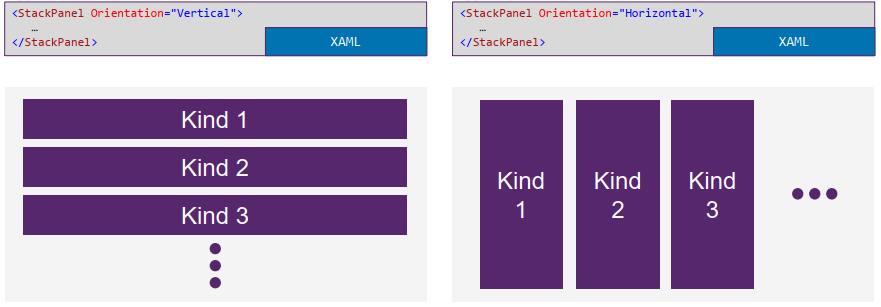
\includegraphics[scale=0.4]{images/stackpanel.PNG}\\
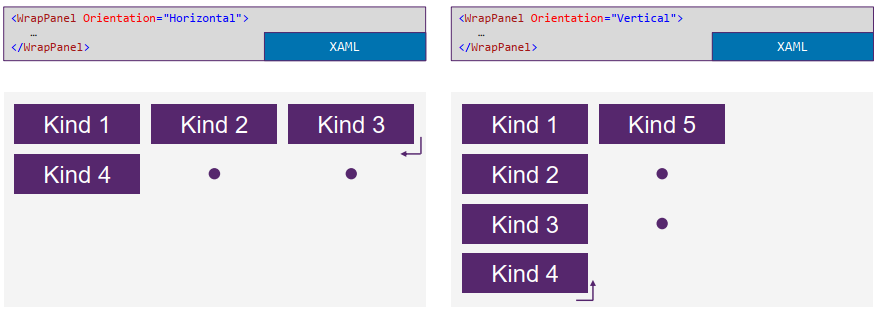
\includegraphics[scale=0.4]{images/wrappanel.PNG}\\
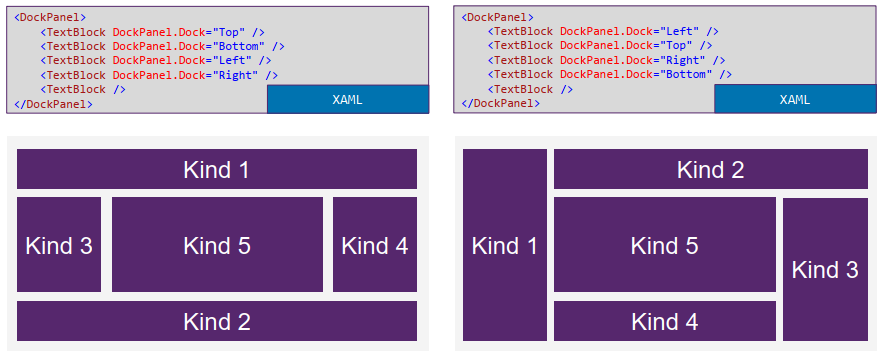
\includegraphics[scale=0.4]{images/dockpanel.PNG}\\
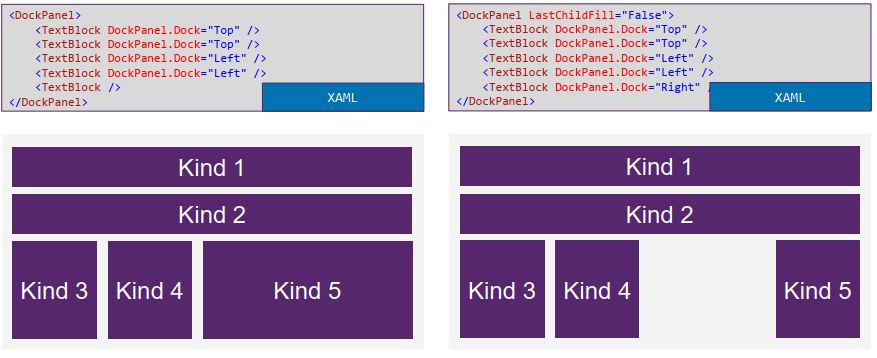
\includegraphics[scale=0.4]{images/dockpanel2.PNG}\\
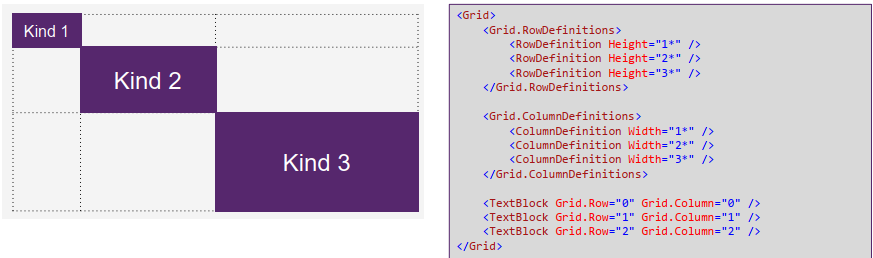
\includegraphics[scale=0.4]{images/grid1.PNG}\\
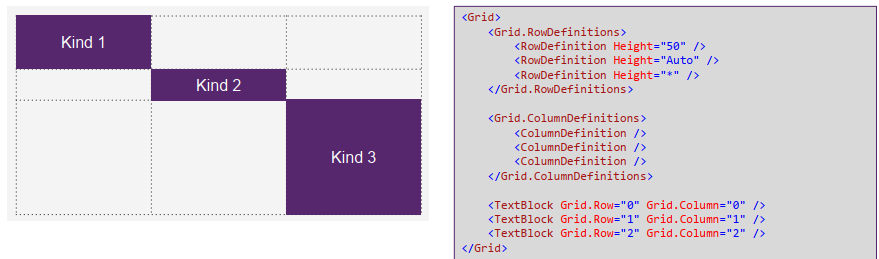
\includegraphics[scale=0.4]{images/grid2.PNG}\\

\subsubsection{Grid}
Breiten- und Höhenangaben\\
• MinWidth und MinHeight\\
• MaxWidth und MaxHeight\\
• Kombinierbar mit Auto- und *-Grössen\\
Zellen und Reihen verbinden\\
• RowSpan und ColSpan\\
Grid erlaubt Stapelung von Elementen\\
• Mehrere Elemente innerhalb einer Zelle\\
• Unten im Layout = oben beim Zeichnen

\section{Controls}
Das Aussehen von Controls wird über Attribute beeinflusst\\
• Grössenangaben mit verschiedenen Dimensionen\\
• Ränder, Innen- und Aussenabstände\\
• Ausrichtungen im Eltern-Element und der Kind-Elemente\\
• Farben und Schriften

\subsection{Image}
Bilddatei zum Projekt hinzufügen\\
• Build Action: Resource\\
• Integration in Binärdatei des Projekts\\
Source für Dateipfad\\
• Relativer Pfad beginnend bei XAML-Datei\\
• Verwendung von Ordnern möglich\\
Stretch für Kontrolle der Skalierung\\
• Uniform: Bildverhältnis beibehalten (Standard)\\
• Fill: Fläche füllen, Bildverhältnis ignorieren\\
• UniformToFill: Fläche füllen, Bildverhältnis beibehalten\\
• None: Bild gemäss Originalgrösse darstellen

\subsection{Border}

Container für genau ein Element\\
• Controls oder Layouts\\
Verwendung zur Gruppierung oder Hervorhebung von Inhalten via …\\
• Rahmen\\
• Hintergrundfarbe\\
• Runde Ecken\\
• Sichtbarkeit

\subsection{Canvas}
2D-Zeichenfläche für einfache geometrische Objekte (Shapes)\\
Absolute Positionierung in X/Y-Raster, keine dynamischen Grössen\\
• Keinerlei Layout-Logik\\
• Kind-Elemente erhalten Attached Properties
\begin{minted}{xml}
<Canvas>
    <Rectangle Canvas.Left="40" Canvas.Top="60"
    Width="128" Height="80" Fill="#006AA6" />
    <Ellipse Canvas.Left="220" Canvas.Top="160"
    Width="120" Height="120" Fill="#6E1C50" />
    <Path Canvas.Left="80" Canvas.Top="64" Width="260"
    Height="200" Stroke="DarkGray" Stretch="Fill"
    Data="M1,0 L0,1"/>
</Canvas>
\end{minted}
Shapes verwenden intern leichtgewichtige Model-Klassen für Geometrieberechnungen\\
Diese können auch selbst verwendet werden, beispielsweise für Window Clipping

\subsection{Window Clipping}
Die Form eines Window kann mittels Clipping beliebig verändert werden\\
Das Window muss dazu jedoch korrekte Einstellungen haben\\
Braucht auf dem Window:
\begin{minted}{xml}
AllowsTransparency="True"
WindowStyle="None
    ...
<Window.Clip>
    <RectangleGeometry RadiusX="30"
                       RadiusY="30" Rect="0,0,400,200" />
</Window.Clip>
\end{minted}
\section{Resources}
\textbf{Ziel}: Objekte zentral definieren und n-fach wiederverwenden\\
Beliebige Objekte, die in XAML definiert werden können\\
• Brush\\
• Color\\
• String\\
Besitzen eine eindeutige Identifikation\\
• Zuweisung des XAML-Attributs x:Key\\
• Erlaubt die spätere Referenzierung
\subsection{Resource Dictionary}
Container zur Speicherung von Resources\\
Zugriff über Schlüssel der Resource (x:Key)\\
Teil aller FrameworkElement-Ableitungen\\
• Zugriff über Property Element Syntax\\
Beispiele\\
• Application.Resources\\
• Window.Resources\\
• Button.Resources\\
• Label.Resources

\begin{minted}{xml}
<Label><Label.Background>
    <StaticResource ResourceKey="OSTBrush" />
</Label.Background></Label>
\end{minted}
\xml{<Label Background="{StaticResource OSTBrush}" />}

\subsection{Auflösung von Resources}
Suchreihenfolge\\
1. Aktuelles Element und alle Parent-Elemente (aufwärts entlang dem Logical Tree)\\
2. In Application.Resources\\
3. In System-Ressourcen\\
Die Suche bricht beim ersten Treffer ab\\
• Reihenfolge im XAML entscheidend\\
• Vorsicht bei mehrfach verwendeten Schlüsseln

\subsection{Statische und dynamische Resourcen}

\textbf{Statische Resources}\\
• Einmalige Auswertung der Resource\\
• Auswertung bei Kompilierung\\
• Unveränderlich zur Laufzeit\\
• Extension: \xml{{StaticResource Key}}\\
\textbf{Dynamische Resources}\\
• Mehrfache Auswertung der Resource\\
• Auswertung bei Ausführung\\
• Veränderlich zur Laufzeit\\
• Extension: \xml{{DynamicResource Key}}

\begin{minted}{xml}
<Window.Resources>
    <SolidColorBrush x:Key="OSTBrush" Color="#6E1C50" />
</Window.Resources>
<StackPanel>
    <Label Content="OK" Foreground="White"
            Background="{DynamicResource OSTBrush}" />
    <Button Content="Update" Click="UpdateResource" />
</StackPanel>
\end{minted}
\begin{minted}{csharp}
private void UpdateResource(object sender, RoutedEventArgs e) {
    Resources["OSTBrush"] = new SolidColorBrush(Colors.Blue);
}
\end{minted}
\subsection{Beliebige Typen?}
• Ein Resource Dictionary nimmt alle Elemente auf, die in XAML definierbar sind\\
• Häufig werden Basistypen benötigt (String, Zahlen)\\
• Diese können in XAML definiert werden\\
\xml{<Window xmlns:s="clr-namespace:System;assembly=System.Runtime">}

\subsection{x:Static – Zugriff auf CLR-Werte}
• Gelegentlich ist es nötig, auf statische Werte der CLR zuzugreifen\\
• Konstanten im eigenen C\#-Code\\
• Konstanten aus .NET\\
\textbf{Zugriff via Markup Extension: x:Static}\\
• Keine WPF-Resources\\
• Werte definiert in normalen Klassen

\begin{minted}{csharp}
public static class MyRes {
    public static SolidColorBrush OSTBrush =
    new SolidColorBrush(Color.FromRgb(110, 28, 80));
}
\end{minted}
\begin{minted}{xml}
<Label Content="x:Static"
Background="{x:Static local:MyRes.OSTBrush}"
Foreground="{x:Static SystemColors.ControlLightBrush}"
FontFamily="{x:Static SystemFonts.CaptionFontFamily}"
FontSize="{x:Static SystemFonts.CaptionFontSize}" />
\end{minted}

\subsection{Eigenständige Resource Dictionaries}
• Separate .xaml-Datei mit XML-Root \xml{<ResourceDictionary>}\\
• In andere Dictionaries als Merged Dictionaries integrierbar\\
• Dictionaries in einem Startup-Event-Handler der App-Klasse laden

\subsection{Externe Resources}
Dictionaries können aus anderen Assemblies eingebunden werden\\
• Verwendung bei umfangreicheren Apps mit mehreren Projekten\\
• Verwendung bei 3rd Party Libraries wie MahApps.Metro\\
Mit \xml{siteOfOrigin} werden Resources im Dateisystem referenziert\\
• Nützlich, wenn Resources erst zur Laufzeit bekannt sind\\
• Austauschen von Resources ohne Neukompilierung der App\\
• Pfad relativ zur ausgeführten .exe-Datei

\subsection{Grenzen von Resources}
Mit Resources können mehrfach verwendete Werte zentral verwaltet werden\\
\textbf{Aber}: wir müssen die Werte weiterhin bei jedem Element referenzieren\\
Das ist besonders ungünstig, wenn Werte für alle Elemente einer Applikation gelten sollen

\subsection{Explizite Styles}
Variante 1: Ohne Angabe des Typs
\begin{minted}{xml}
<Style x:Key="MyButtonStyle">
<Button Style="{StaticResource MyButtonStyle}"
\end{minted}
Variante 2: Mit Angabe des Typs
\begin{minted}{xml}
<Style x:Key="MyButtonStyle" TargetType="Button">
\end{minted}
\subsection{Implizite Styles}
\begin{minted}{xml}
<Style TargetType="Button">
<!--Style erhält automatisch den Key x:Key="{x:Type Button}"-->
\end{minted}

\subsection{Styles erweitern}
Styles sind mit Inline-Attributen kombinierbar\\
• Eignet sich für einmalige Anpassungen, z.B. das Hervorheben eines bestimmten Buttons\\
Styles können auch vererbt werden\\
• Eine clevere Hierarchie kann den Umfang der Resourcen stark reduzieren
\begin{minted}{xml}
<Style x:Key="NormalButton" TargetType="Button">
    ...
</Style>
<Style x:Key="DangerButton"
    BasedOn="{StaticResource NormalButton}" TargetType="Button">
    <Setter Property="Background" Value="Red" />
</Style>
\end{minted}
\subsection{Komplexe Werte}
Komplexe Werte in Styles sind über die Property Element Syntax möglich\\
• Setzen des Value-Attributs auf dem Setter-Element\\
• Ansonsten selbe Syntax wie im normalen XAML
\begin{minted}{xml}
<Style x:Key="BrushButton" TargetType="Button">
    <Setter Property="Background">
        <Setter.Value>
            <LinearGradientBrush StartPoint="0,0" EndPoint="0,1">
                <GradientStop Offset="0" Color="Red" />
                <GradientStop Offset="0.5" Color="Yellow" />
                <GradientStop Offset="1" Color="Red" />
            </LinearGradientBrush>
</Setter.Value></Setter></Style>
\end{minted}

\subsection{Trigger}
Trigger erlauben Stylings basierend auf dem Zustand eines Elementes\\
• Beliebige Attribute des Elements sind auswertbar\\
• Achtung: einige Elemente besitzen standardmässig bereits Trigger (z.B. Button)
\begin{minted}{xml}
<Style.Triggers>
    <Trigger Property="Content" Value="Link">
        <Setter Property="Cursor" Value="Hand" />
    </Trigger>
    <Trigger Property="Content" Value="Edit">
        <Setter Property="Cursor" Value="Pen" />
    </Trigger>
</Style.Triggers>
\end{minted}

\subsection{Skins / Themes}
WPF kennt kein Skin- oder Theme-Konzept\\
Kann mit den bestehenden Mechanismen aber problemlos nachgebaut werden\\
• Mehrere Dateien mit gleichen benannten Styles darin\\
• Laden des gewünschten Resource Dictionaries zur Laufzeit\\
• Zuweisung der Styles über DynamicResource


\section{Control Templates}
Control Templates beschreiben die visuelle Repräsentation von XAML-Controls\\
• Elemente, die im Visual Tree eingefügt werden\\
Der Zugriff auf das aktuelle Template erfolgt\\
über das Attribut Control.Template\\
• Standard-Template pro Control vorhanden\\
• Eigene Templates möglich\\
Eigene Control Templates\\
• Option 1: Als ControlTemplate-Resource\\
• Option 2: Innerhalb eines Styles
\begin{minted}{xml}
<Border BorderBrush="{TemplateBinding BorderBrush}">
    ...
    <ContentPresenter Content="{TemplateBinding Content}"
    Margin="5 0 10 0" VerticalAlignment="Center" />
</Border> 
<Button Grid.Row="0" Content="Button mit Template"
Template="{StaticResource ButtonTemplate}"/>
\end{minted}
Control Templates\\
\xml{ContentPresenter}\\
• Platzhalter für den Content des Elementes\\
• Verwendung optional, aber sehr zu empfehlen\\
\xml{TemplateBinding}\\
• Markup Extension für das Binding an Attribute\\
• Nur in Control Templates verwendbar

\textbf{Keine WPF Design Guidelines}\\
Empfehlung: Guidelines und Libraries nutzen, die sich andernorts bewährt haben

\section{Databinding}
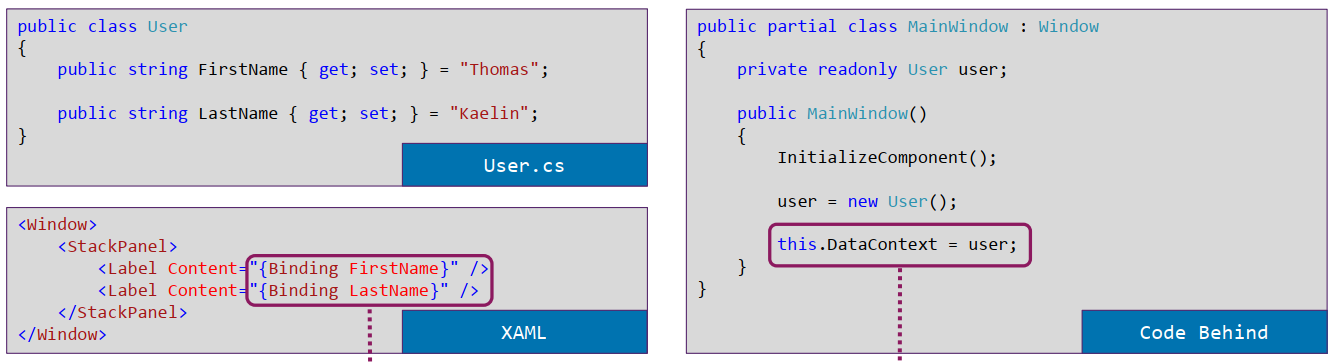
\includegraphics[scale=0.3]{images/Databinding.PNG}
\subsection{Bindings}
Verknüpfen Ziel und Quelle miteinander\\
• Binding für 1:1 Verknüpfungen\\
• MultiBinding für 1:n Verknüpfungen\\
• PriorityBinding für 1:n / 1:1 Verknüpfungen\\
Varianten zur Erzeugung von Bindings\\
• Attribute Syntax + Markup Extension\\
• Property Element Syntax\\
• C\# Code\\
Ziel-Eigenschaften müssen Dependency Properties sein\\
• Erweiterte CLR-Properties für WPF

Path\\
• Name der Quell-Eigenschaft\\
• Objektpfad-Syntax möglich (z.B. x.y.z)\\
• Standardparameter der Markup Extension\\
Mode\\
• Richtung des Datenflusses\\
• Standardwert abhängig von Ziel-Eigenschaft\\
Converter\\
• Datenumwandlung zwischen Quelle und Ziel\\
• Umwandlung in beide Richtungen möglich

\begin{minted}{xml}
<Binding Path="FirstName" Mode="TwoWay"
    Converter="{StaticResource MyCnv}" />}
\end{minted}   
\subsection{Mode}
• OneTime Einmalige Aktualisierung des Ziels beim Setzen der Quelle\\
• OneWay Ziel wird bei Änderungen der Quelle aktualisiert\\
• OneWayToSource Quelle wird bei Änderungen des Zieles aktualisiert\\
• TwoWay Änderungen werden in beide Richtungen propagiert\\
• Default Wert abhängig von Ziel-Eigenschaft

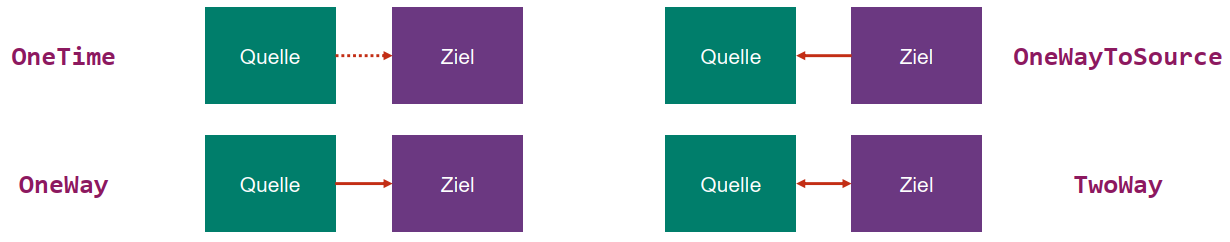
\includegraphics[scale=0.29]{images/Bindings.PNG}

\subsection{Value Converter}
Datenumwandlung zwischen Quelle und Ziel\\
• Beispiel 1: bool zu Visibility\\
• Beispiel 2: Strings umformatieren\\
Interface IValueConverter\\
• Convert(…) Quelle zu Ziel\\
• ConvertBack(…) Ziel zu Quelle\\
Erzeugung von Converter\\
• Option 1: In Resources (StaticResource)\\
• Option 2: In Code (x:Static)

\begin{minted}{csharp}
public class ReverseConverter : IValueConverter {
    public object Convert(object value, ...) {
        var stringValue = (string) value;
        var reversedChars = stringValue.Reverse().ToArray();
        var reversedString = new string(reversedChars);
        return reversedString;
    }
    public object ConvertBack(object value, ...) {
        return Convert(value, ...);
}}
\end{minted}


\includegraphics[scale=0.3]{images/Converter.PNG}

\subsection{Weitere Eigenschaften}
\csharp{Delay} Verzögerung in Millisekunden bei Updates vom Ziel zu Quelle\\
\csharp{StringFormat} Formatangabe für Bindings mit dem Zieltyp string\\
\csharp{FallbackValue} Ergebnis, wenn Binding fehlschlägt (z.B. falscher Pfad)\\
\csharp{TargetNullValue} Ergebnis, wenn Quell-Eigenschaft null liefert\\
\csharp{UpdateSourceTrigger} Zeitpunkt, zu welchem das Quell-Element aktualisiert wird. Mit Explicit selbst laden.\\
z.B. LostFocus oder PropertyChanged; Standard abhängig vom Ziel

\subsection{Multi Binding}
Verwendung analog zu Binding\\
• Path, Mode, Converter, etc.\\
Unterschiede\\
• Beliebig viele Quell-Eigenschaften\\
• Nur Property Element Syntax (oder C\# Code)\\
• Converter mit IMultiValueConverter\\
Je nach Ziel-Eigenschaft ist ein Converter zwingend nötig (z.B. Label.Content)
\begin{minted}{xml}
<MultiBinding StringFormat="{}{0} {1} ({2} Jahre)">
    <Binding Path="FirstName" />
    <Binding Path="LastName" />
    <Binding Path="Age" />
</MultiBinding>
\end{minted}

\subsection{Data Context}
Property der Klasse FrameworkElement\\
Setzt die Standardquelle für Bindings\\
Falls undefiniert: Traversierung des Logical Trees nach oben bis zum ersten Treffer\\
Jeder Path ist relativ zum DataContext\\
Beliebige Objekte möglich\\
• C\#-Klassen, WPF-Elemente, etc.\\
• Typischerweise: View Models

\subsubsection{überschreiben}
Der Data Context lässt sich für einzelne Elemente anpassen\\
• Option 1: Im Code Behind das Property\\
DataContext für das Element setzen\\
• Option 2: Source im Binding setzen\\
Dies ist eher unüblich – meist wird ein Data Context pro Window verwendet

\begin{minted}{csharp}
public MainWindow() {
    InitializeComponent();
    var user = new User();
    this.LastNameLabel.DataContext = user;
    this.FirstNameLabel.DataContext = user;
}
\end{minted}
\begin{minted}{xml}
<Window.Resources>
    <local:User x:Key="MyUser" />
</Window.Resources>
<Label Content="{Binding Source={StaticResource MyUser},
Path=FirstName}" />
\end{minted}
\subsection{Weitere Quellen}
Mit \csharp{RelativeSource} werden Elemente im Visual Tree referenziert\\
• Markup Extension \xml{{RelativeSource ...}}\\
• Suche beginnt beim definierenden Element\\
• Beispiel: Binding an die Eigenschaft Title des beinhaltenden Window-Objektes\\
\begin{minted}{xml}
<Label Content="{Binding RelativeSource={RelativeSource
FindAncestor, AncestorType=Window}, Path=Title}" />
\end{minted}
Mit \csharp{ElementName} werden Elemente über Namen referenziert\\
• Namen müssen im gleichen Namensraum vorliegen\\
• Beispiel: Binding an die Eigenschaft Text des Objektes mit Name MyText
\begin{minted}{xml}
<TextBox Name="MyText" Text="Hallo MGE" />
<TextBox Text="{Binding ElementName=MyText, Path=Text}" />
\end{minted}

\subsubsection{Design Time Support}
Der XAML Designer kennt den Typ des Objekts im Data Context standardmässig nicht\\
• Das heisst: keine Autovervollständigung verfügbar (IntelliSense)\\
Als Abhilfe kann das Attribut d:DataContext beim Window gesetzt werden\\
• Variante 1: Objekterzeugung in XAML und Markup Extension 
\xml{{d:DesignInstance ...}}
\begin{minted}{xml}
d:DataContext="{
d:DesignInstance Type=local:User,IsDesignTimeCreatable=True}"
\end{minted}
• Variante 2: Objekterzeugung in C\# und Markup Extension \xml{{x:Static …}}
\begin{minted}{xml}
d:DataContext="{x:Static local:DesignerData.User}
\end{minted}

\section{Aktualisierung von Daten}
\subsection{POCOs als Data Context}

Als Datenquelle können beliebige Objekte verwendet werden, also auch POCOs*\\
Unsere Bindings funktionieren – allerdings nur mit Einschränkungen (siehe Beispiel)\\
Mögliche Lösungen\\
• Observer Pattern\\
• Observables bei Data Binding\\
Die Observer-Variante in .NET heisst\\
INotifyPropertyChanged
\begin{minted}{xml}
<Window>
    <Label Content="{Binding Age}" />
    <Button Content="Alter ++" Click="Increment" />
</Window>
\end{minted}
\begin{minted}{csharp}
public partial class MainWindow : Window {
    private readonly User user;
    private void Increment(object sender, RoutedEventArgs e) {
        user.Age++;
}}
public class User {
    public string FirstName { get; set; } = "Thomas";
    public string LastName { get; set; } = "Kaelin";
    public int Age { get; set; } = 36;
}
\end{minted}
\subsection{INotifyPropertyChanged}
Bestandteil des .NET Framework\\
• Interface mit nur einem Event\\
• Name des geänderten Property in EventArgs\\
\begin{minted}{csharp}
public interface INotifyPropertyChanged {
    event PropertyChangedEventHandler PropertyChanged;
}
public delegate void PropertyChangedEventHandler(
object sender, PropertyChangedEventArgs eventArgs);
public class PropertyChangedEventArgs : EventArgs {
    public PropertyChangedEventArgs(string propertyName) {
        this.PropertyName = propertyName;
    }
    public virtual string PropertyName { get; }
}
\end{minted}
\subsubsection{Ohne Hilfmittel}
\begin{minted}{csharp}
public class User : INotifyPropertyChanged {
private string _firstName = "Thomas";
    public string FirstName {
        get => _firstName;
        set {
            if (_firstName != value) {
                _firstName = value;
                OnPropertyChanged(nameof(FirstName));
    }}}
    public event PropertyChangedEventHandler PropertyChanged;
    protected virtual void OnPropertyChanged(string name) {
        var eventArgs = new PropertyChangedEventArgs(name);
        PropertyChanged?.Invoke(this, eventArgs);
}}
\end{minted}

\subsubsection{Mit Hilfmittel}
\begin{minted}{csharp}
public abstract class BindableBase : INotifyPropertyChanged {
    public event PropertyChangedEventHandler PropertyChanged;
    protected virtual void OnPropertyChanged(string name) {
        var eventArgs = new PropertyChangedEventArgs(name);
        PropertyChanged?.Invoke(this, eventArgs);
    }
    protected bool SetProperty<T>(ref T field, T value,
    // Compilezeit name des Porperties
    [CallerMemberName] string name = null) { 
        if (Equals(field, value))
            return false;
        field = value;
        OnPropertyChanged(name);
        return true;
}}
public class User : BindableBase {
    private string _firstName = "Thomas";
    public string FirstName {
        get => _firstName;
        set => SetProperty(ref _firstName, value, nameof(FirstName));
}}
\end{minted}

\subsubsection{Fody}
Fody basiert auf IL Weaving\\
• Anpassung der IL zum Kompilationszeitpunkt\\
• Fody «webt» aufgrund bestimmter Kriterien dynamisch IL Code ein\\
\\
PropertyChanged.Fody\\
• Vereinfacht INPC-Implementierungen\\
• Wandelt normale Properties automatisch um\\
• Verfügbar als NuGet-Paket
\subsection{Anmerkungen}
Vorsicht bei zusammengesetzten Eigenschaften (z.B. FullName => FirstName + LastName)\\
• Event für FullName muss bei jeder Änderung von FirstName oder LastName ausgelöst werden\\
• Das kann ganz schön kompliziert werden\\
• Einige Libraries – wie Fody – helfen auch hierbei\\
Unsere Model-Klassen sollten idealerweise keine technologischen Details enthalten\\
• Dazu zählt auch die Implementierung von INPC\\
• Üblicherweise implementiert das View Model INPC – so bleibt das Model «sauber»

\section{Collections}
\subsection{Datenbindung an Collections}
Bisher haben wir nur «einfache» Objekte gebunden – was bei Collections?\\
Quelle muss INotifyCollectionChanged implementieren\\
Die Ziel-Eigenschaft muss eine Collection erwarten\\
Solche Eigenschaften haben Elemente, die der Darstellung von Collections dienen


\subsection{INotifyCollectionChanged}
Bestandteil des .NET Framework\\
• Enthält – wie INPC – ebenfalls nur ein Event\\
• Collection-Änderung in Event Args beschrieben (Hinzufügen, Löschen, etc.)\\
\csharp{ObservableCollection<T>}\\
• Implementiert INPC und INCC\\
• Eigene Implementierung von INCC seltener

\subsection{ItemsControl}
• Wichtigste Basisklasse für WPF-Elemente zur Anzeige von Collections\\
• Definiert folgende Ziel-Eigenschaften (Auswahl)\\
• Items – Enthält angezeigte Elemente\\
• ItemsSource – Füllt Inhalt über Data Binding ab\\
• ItemTemplate – Definiert das Template für die Darstellung eines Items\\

\textit{Bei Verwendung von \csharp{ItemsSource} wird \csharp{Items} zu einer
read-only Eigenschaft umgewandelt.  \underline{Keine Kombination!}}\\
\textit{Represents a control that can be used to present a collection of items}
\begin{minted}{csharp}
public partial class MainWindow : Window {
    private ObservableCollection<User> users;
    public MainWindow() {
        InitializeComponent();
        // Die Collection müsste natürlich befüllt werden…
        users = new ObservableCollection<User>();
        this.DataContext = users;
}}
public class User {
    public string FirstName { get; set; } = "Thomas";
    public string LastName { get; set; } = "Kaelin";
}
\end{minted}
\begin{minted}{xml}
<Window>
    <ListBox ItemsSource="{Binding}">
        <ListBox.ItemTemplate>
            <DataTemplate>
                <StackPanel>
                    <TextBlock Text="{Binding LastName}"/>
                    <TextBlock Text="{Binding FirstName}"/>
                </StackPanel>
</DataTemplate></ListBox.ItemTemplate></ListBox></Window>
\end{minted}
\subsection{Item Template als Resource}
Das Item Template kann als Resource definiert werden\\
Das Template ist so wiederverwendbar und der XAML Code schlanker\\
Durch das Attribut DataType ist IntelliSense gewährleistet
\begin{minted}{xml}
<Window.Resources>
    <DataTemplate x:Key="UserTemplate" DataType="local:User">
        <StackPanel>
            <TextBlock Text="{Binding LastName}"/>
            <TextBlock Text="{Binding FirstName}"/>
</StackPanel></DataTemplate></Window.Resources>
<ListBox ItemsSource="{Binding}"
    ItemTemplate="{StaticResource UserTemplate}" />
\end{minted}
\subsection{Selector}
Erweitert ItemsControl um Logik zur Selektion von Elementen\\
Definiert folgende wichtigen Eigenschaften (Auswahl)\\
• \csharp{SelectedIndex} – Index des ausgewählten Elements\\
• \csharp{SelectedItem} – Ausgewähltes Element als Objekt\\
• \csharp{SelectedValue} – Wert des ausgewählten Elements\\
• \csharp{SelectedValuePath} – Objektpfad-Syntax zum Wert, der in \csharp{SelectedValue} zurückgeliefert wird\\

\textit{Represents a control that allows a user to select items from among its child elements.}
\begin{minted}{xml}
<ListBox ItemsSource="{Binding Users}"
        ItemTemplate="{StaticResource UserTemplate}"
        SelectedIndex="{Binding SelectedUserIndex}"
        SelectedItem="{Binding SelectedUser}"
        SelectedValue="{Binding SelectedUserFirstName}"
        SelectedValuePath="FirstName" />
\end{minted}
\begin{minted}{csharp}
public partial class MainWindow : Window {
    public ObservableCollection<IUser> Users { get; }
    public IUser SelectedUser { get; set; }
    public int SelectedUserIndex { get; set; }
    public string SelectedUserFirstName { get; set; }
    public MainWindow() {
        InitializeComponent();
        // Wie gehabt – hier irgendwie „Users“ befüllen
        this.DataContext = this;
}}
\end{minted}
\section{MVVM im Überblick}
Ziel: Trennung von Präsentation und Logik\\
\textbf{Model} umfasst Domänen-/Businesslogik\\
• C\# Klassen (ggf. mit INPC oder INCC)\\
• Oft durch Interfaces abstrahiert\\
\textbf{View} kümmert sich um die Darstellung\\
• XAML\\
• Code Behind\\
\textbf{View Model} enthält Darstellungslogik\\
• C\# Klasse mit INPC

\subsection{V - View}
\textbf{Kümmert sich um die Darstellung}\\
• Sollte möglichst «dumm» sein\\
• Logik und Zustände gehören ins View Model\\
\textbf{Bedeutung «dummer Views»}\\
• Faustregel: Die Applikation sollte vollständig über das View Model bedienbar sein (z.B. mit Tests)\\
• Beispiel 1: Verarbeitung von Selektionen im View Model (z.B. SelectedItem)\\
• Beispiel 2: Steuerung von Sicht- und Verfügbarkeiten durch das View Model\\
\textbf{Prinzipien des Software Engineerings auch für die View anwenden}\\
• Clean Code (DRY, KISS, YAGNI, SOLID, etc.)\\
• Beispiel 1: Definition von wiederverwendbaren Styles anstelle von Inline-Attributen\\
• Beispiel 2: Auslagern von Item Templates als Resources zur besseren Lesbarkeit\\

Bestandteile in WPF: XAML, Code Behind, Resources, Value Converter, Markup Extensions, Eigene Controls

\subsection{VM – View Model}
Enthält komplette Logik der Darstellung\\
Typische Aufgaben\\
• Formatierung von Model-Eigenschaften\\
• Halten von Zuständen\\
• Validierung von Benutzereingaben\\
• Delegation von Benutzeraktionen an Model\\
Bestandteile in WPF\\
• C\#-Klassen mit INPC

\section{View Models in WPF}
\subsection{Beispiel Klassisch}
\begin{minted}{csharp}
public partial class UserView : Window {
    public UserView() {
        InitializeComponent();
        var user = new User();
        DataContext = new UserViewModel(user);
    }
}
public class UserViewModel : BindableBase {
    private string _first;
    private string _last;
    public UserViewModel(User user) {
        _first = user.FirstName;
        _last = user.LastName;
    }
    public string FirstName {
        get => _first;
        set {
            if (SetProperty(ref _first, value)) {
                OnPropertyChanged(nameof(FormattedName));
    }}}
    public string LastName { ... } // Analog zu FirstName
    public string FormattedName => "{_first} {_last}";
}
\end{minted}
\begin{minted}{xml}
<Window>
    <StackPanel>
        <TextBox Text="{Binding FirstName}" />
        <TextBox Text="{Binding LastName}" />
        <TextBlock Text="{Binding FormattedName}" />
    </StackPanel>
</Window>
\end{minted}
\subsection{Beispiel Durchgriff}
\begin{minted}{csharp}
public class User : BindableBase {
    private string _firstName = string.Empty;
    private string _lastName = string.Empty;
    public string FirstName {
        get => _firstName;
        set => SetProperty(ref _firstName, value);
    }
    public string LastName {
        get => _lastName;
        set => SetProperty(ref _lastName, value);
}}
public class UserViewModel : BindableBase {
    private User _user;
    public UserViewModel(User user) {
        User = user;
    }
    public IUser User {
        get => _user;
        private set => SetProperty(ref _user, value);
}}
\end{minted}
\begin{minted}{xml}
<StackPanel>
    <TextBox Text="{Binding User.FirstName}" />
    <TextBox Text="{Binding User.LastName}" />
    <TextBlock>
        <TextBlock.Text>
            <MultiBinding StringFormat="{}{0} {1}">
                <Binding Path="User.FirstName" />
                <Binding Path="User.LastName" />
</MultiBinding></TextBlock.Text></TextBlock></StackPanel>
\end{minted}

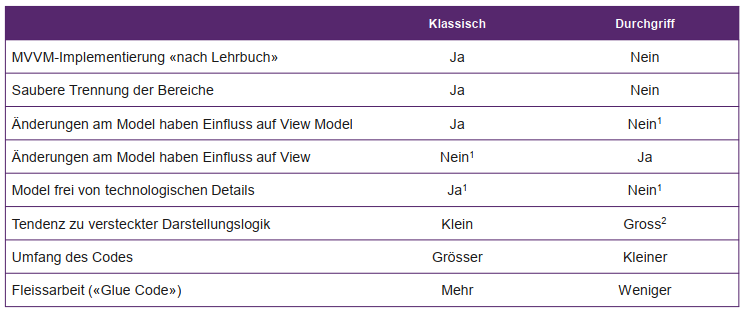
\includegraphics[scale=0.45]{images/MVVM_Klasisch_Durchgriff.PNG}

\subsection{AutoMapper- «Klassisch» verbessert}
Hauptnachteil der Variante «Klassisch» ist der zusätzliche Glue Code
AutoMapper entschärft das Problem
• Objekt-Objekt-Mapper (O/O-Mapping)
• Abfüllen des View Models aus dem Model(und bei Bedarf zurück)
• Integration als NuGet-Paket
• Beispiel: View Model aus Model erzeugen
\begin{minted}{csharp}
var config = new MapperConfiguration(cfg => 
             cfg.CreateMap<User, UserViewModel>());
var mapper = config.CreateMapper();
var viewModel = mapper.Map<UserViewModel>(user);
\end{minted}

\subsection{Aktionen in View Models}
Data Binding erlaubt die Verknüpfung von Eigenschaften, nicht aber von Method\\
Methoden müssen in Objekte verpackt werden\\
• ICommand definiert die Schnittstelle für solche Objekte\\
• View Models stellen ICommand-Objekte zur Verfügung\\
Command-Eigenschaft von Controls wird an ICommand-Objekte gebunden\\
• Button\\
• CheckBox\\
• RadioButton

\subsection{ICommand}
\csharp{Execute(Object parameter)}\\
• Enthält den Code der auszuführenden Aktion\\
• Beispiel: Alter eines Benutzers verringern\\
\csharp{CanExecute(Object parameter)}\\
• Prüft, ob die Aktion ausgeführt werden kann\\
• Steuert bei einigen Controls die Verfügbarkeit (IsEnabled)\\
• Beispiel: true, falls Alter grösser als 0, sonst false\\
\csharp{CanExecuteChanged}\\
• Auszulösen, wenn Bedingung in CanExecute() sich ändert\\
• Beispiel: Nach jeder Änderung des Alters

\subsubsection{Beispiel 1 – Ohne Hilfsmittel}
\begin{minted}{csharp}
public class DecreaseAgeCommand : ICommand {
    private readonly UserViewModel _viewModel;
    public DecreaseAgeCommand(UserViewModel viewModel) {
        _viewModel = viewModel;
    }
    public bool CanExecute(object parameter) {
        return _viewModel.Age > 0;
    }
    public void Execute(object parameter) {
        _viewModel.Age--;
        OnCanExecuteChanged();
    }
    public event EventHandler CanExecuteChanged;
    protected virtual void OnCanExecuteChanged() {
    CanExecuteChanged?.Invoke(this, EventArgs.Empty);
}}
public class UserViewModel : BindableBase {
    public UserViewModel(User user) {
        DecreaseAgeCommand = new DecreaseAgeCommand(this);
    }
    public int Age {get => {};set => {};}
    public ICommand DecreaseAgeCommand { get; }
}
\end{minted}
\begin{minted}{xml}
<Window>
    <StackPanel>
        <Button Content="Decrease Age"
        Command="{Binding DecreaseAgeCommand}" />
</StackPanel></Window>
\end{minted}

\subsubsection{Beispiel 2 – Mit Hilfsklasse}
\begin{minted}{csharp}
public sealed class RelayCommand : ICommand {
    private readonly Action _execute;
    private readonly Func<bool> _canExec;
    public RelayCommand(Action execute, Func<bool> canExec) {
        _execute = execute;
        _canExec = canExec;
    }
    public bool CanExecute(object parameter) => _canExec();
    public void Execute(object parameter) => _execute();
    public event EventHandler CanExecuteChanged;
    public void RaiseCanExecuteChanged() {
        CanExecuteChanged?.Invoke(this, EventArgs.Empty);
}}
public class UserViewModel : BindableBase {
    public UserViewModel(User user) {
        DecreaseAgeCommand = new RelayCommand(
        OnDecreaseAge, CanDecreaseAge);
    }
    public int Age {get => {};private set => {};}
    public ICommand DecreaseAgeCommand { get; }
    private bool CanDecreaseAge() => Age > 0;
    private void OnDecreaseAge() {
        Age--;
        DecreaseAgeCommand.RaiseCanExecuteChanged();
}}
\end{minted}
\subsection{Relay Command}
Vorteile des Relay Command\\
• ICommand-Interface einmalig implementiert\\
• Universell verwendbar\\
• Command-Code näher beim View Model\\
Nachteile des Relay Command\\
• Keine wiederverwendbaren Command-Klassen\\
-> Theoretisches Problem: Logik in normalen Klassen strukturieren\\
Ein «Relay Command» ist in fast allen Frameworks enthalten\\
• Beispiel: RelayCommand in MVVM Light\\
• Beispiel: DelegateCommand in Prism.WPF\\

\subsection{Commands mit Parametern}
Commands können Parameter übernehmen\\
• \csharp{Execute(Object parameter)}\\
• \csharp{CanExecute(Object parameter)}\\
Der Parameter wird in der View gebunden\\
• Attribut \csharp{CommandParameter}\\
• Typischerweise Binding auf ein Property\\
• Alternativen möglich (z.B. statische Werte)\\
Generisches Relay Command als Hilfsmittel\\
• Prism.WPF: \csharp{DelegateCommand<T>}
\begin{minted}{xml}
<Button Content="Show Details"
Command="{Binding ShowDetailsCommand}"
CommandParameter="{Binding SelectedUser}" />
\end{minted}

\section{Tipps}
\subsection{Zuteilung von Logik:}
Ist die Logik Teil der Domäne oder wird in der Applikation mehrfach verwendet? -> Model\\
Ist die Logik unabhängig vom verwendeten UI Framework? -> View Model\\
Otherwise: View\\
Erzeugung von Views und View Models\\
• Wer erstellt die View Models?\\
• Wer erstellt die Views?\\
Erzeugung des View Models\\
• Erzeugen in View\\
• Dependency Injection über Data Context\\
• Dependency Injection über Konstruktor\\

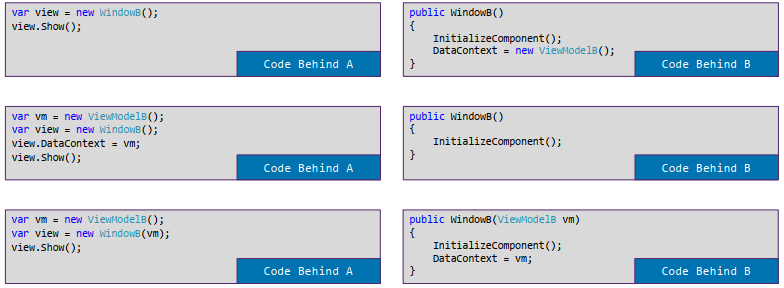
\includegraphics[scale=0.45]{images/ErzeugungVM.PNG}
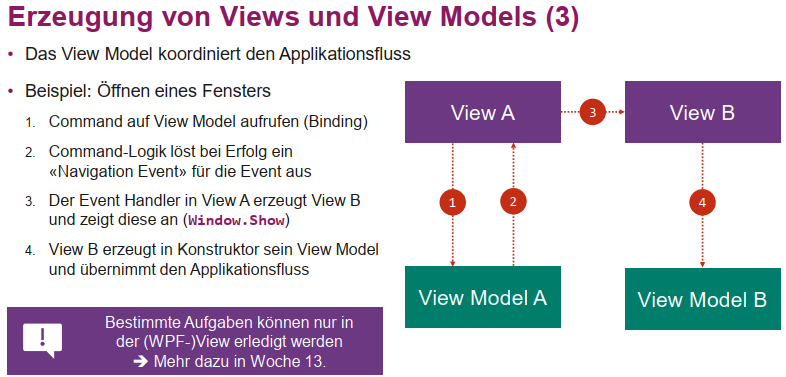
\includegraphics[scale=0.45]{images/ErzeugungVM-2.PNG}

\subsection{MVVM Frameworks in .NET}
\textbf{Prism Library}\\
• Framework für WPF- und Xamarin-Applikationen\\
• Ursprünglich von Microsoft entwickelt, jetzt Open Source\\
\textbf{MVVM Light}\\
• Leichtgewichtiges Toolkit für .NET UI Technologien\\
• 1-Mann Open Source Projekt von Laurent Bugnion\\
\textbf{MvvmCross}\\
• Framework für .NET UI Technologien (insb. Xamarin)\\
• Open Source Projekt bei GitHub

\subsection{Hilfsmittel für das Model – Entity Framework}
• Empfohlene O/R-Mapping-Technologie für .NET Anwendungen\\
• Unterschiedliche Entwicklungsansätze\\
• Model-First Erstellung des Modells in visuellem Editor\\
• Database-First Erstellung der Datenbank mit SQL\\
• Code-First Erstellung des Modells mit attributierten POCO’s

\subsection{Hilfsmittel für das Model – Anderes}
SQLite.net\\
• Einfacher O/R-Mapper auf Basis von SQLite-Datenbanken\\
• Leichtgewichtiger als Entity Framework\\
• Arbeitet ebenfalls mit attributierten POCO’s\\
• Spannend insbesondere für Mobile Apps auf Basis von Xamarin\\
• Integration via NuGet gemäss Anleitung\\
Json.NET / Newtonsoft.Json\\
• Standard-Bibliothek zur Verarbeitung von JSON\\
• Nützlich für Web Services oder die Persistierung von Objekten als JSON-Files\\
• Integration via NuGet gemäss Anleitung

\section{Architektur}
\subsection{Nutzen von Schichten}
Hauptgründe für Schichten\\
• Fachliche, technische oder organisatorische Grenzen\\
• Positiver Einfluss auf SW-Qualitätsmerkmale\\
• Sorgen bei grossen Projekt für Überblick\\
Anzahl und Namen der Schichten sekundär\\
• Unterschiede je nach Technologie\\
• Unterschiede je nach Firma\\
• Unterschiede je nach Architekt\\

\subsection{Horizontale und vertikale Schnitte}
\textbf{Horizontale Schnitte}\\
• Traditioneller Ansatz\\
• Geeignet für «Technologie Teams»\\
• Austausch von Technologien einfacher\\
\textbf{Vertikale Schnitte}\\
• Modernerer Ansatz\\
• Geeignet für «Feature Teams»\\
• Austausch von Technologien schwieriger\\

\subsection{Technologische Grenzen}
Model und View Model sollen technologie-neutral sein\\
• Testbarkeit von Model und View Model\\
• Wiederverwendbarkeit von Model und View Model\\
• Austauschbarkeit von View\\
Schön und gut, aber …\\
• Wie zeigen wir Fehlermeldungen an?\\
• Wie öffnen wir neue Fenster?\\
Generell:\\
• Wie erledigen wir technologie-spezifische Aufgaben?

\subsection{Dependency Injection}
Client kennt Service nur als Interface\\
Injector erzeugt Service und Client\\
Injector injiziert Abhängigkeiten via\\
• Konstruktor\\
• Methode\\
• Property\\

\subsection{Grundmuster für DI}
1. Interface für Verhalten definieren
2. Interface im View Model verwenden
3. Interface im Plattform-Projekt implementieren
4. Service im Plattform-Projekt erzeugen
5. View Model im Plattform-Projekt erzeugen
6. Service in View Model injizieren

\subsection{Vor- und Nachteile von DI}
\textbf{Vorteile}\\
• Geringere Kopplung zwischen Klassen\\
• Zwang zur Separation of Concerns\\
• Austauschbarkeit von Services\\
• Erhöhte Testbarkeit\\
• Weniger Glue Code im Client\\
\textbf{Nachteile}\\
• Zusätzliche Komplexität\\
• Erschwertes Debugging\\
• Parameterlisten bei vielen Abhängigkeiten\\
• Mehr Glue Code beim Injector

\subsection{DI Container}
• Nützlich bei grossen Projekten mit vielen, voneinander abhängigen Services\\
• Kümmern sich um die Erzeugung der Clients mit ihren benötigten Services\\
• Konfiguration des Containers nötig («Mapping von Interface zu Service»)\\
• Lebensdauer konfigurierbar (z.B. Singleton)\\

\subsection{«Clean Architecture»}
Domäne bildet den Kern unserer Software\\
Innere Ringe kennen äussere Ringe nicht\\
Technische «Details» liegen ganz aussen\\
Basiert auf Dependency Injection\\
• Interfaces in den inneren Ringen\\
• Implementierungen in den äusseren Ringen\\
• Konfiguration der Mappings im äussersten Ring\\

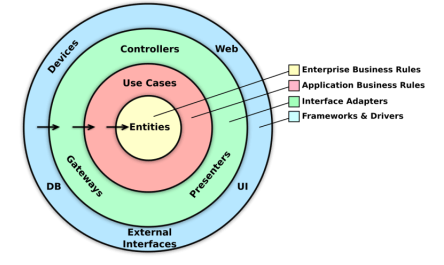
\includegraphics[scale=0.5]{images/kreis.PNG}

\subsection{Testing}
Unit Tests profitieren stark von DI\\
• Test-Projekt als «Plattform-Projekt»\\
• Implementierung von Fake-Services\\
• Injektion von Fake-Services\\
Implementierung von Service\\
• Variante 1: selber implementieren\\
• Variante 2: Mocking Library verwenden\\

\subsection{Klasse Application}
Bisher verwendet als
• Einstiegspunkt in unsere Applikation
• Container für applikationsweite Ressourcen
Statische Eigenschaft Current liefert Singleton-Objekt
• Erlaubt Zugriff von überall auf Properties, Methoden, etc.
• Nützlich für FindResource() und Shutdown()
Lifetime Events
• Innerhalb von Application: Methoden überschreiben
• Ausserhalb von Application: Event Handler registrieren

\subsection{Mehrsprachigkeit – Variante «Resources»}
• Strings in Resource Dictionaries\\
• Pro Sprache eine XAML-Datei\\
• Zugriff im XAML über {DynamicResource …}\\
• Zugriff in C\# über FindResource()\\
• Anpassen der Resource Dictionaries bei Sprachänderung im Code Behind

\begin{minted}{xml}
<ResourceDictionary>
    <system:String x:Key="Key1">Translation 1</system:String>
</ResourceDictionary>

<Window>
    <Label Content="{DynamicResource Key1}" />
</Window>
\end{minted}

\begin{minted}{csharp}
public void LoadTranslations(string key) {
    var uri = new Uri("/MyApp;component/Trans.{key}.xaml",
    UriKind.RelativeOrAbsolute);
    var rd = new ResourceDictionary { Source = uri };
    foreach (var rdKey in rd.Keys) {
        Resources[rdKey] = rd[rdKey];
}}
\end{minted}
\subsection{Mehrsprachigkeit – Variante «RESX»}
Strings in RESX-Dateien\\
Pro Sprache eine RESX-Datei\\
Zugriff im XAML über {x:Static …}\\
Zugriff in C\# über generierte Klasse\\
Anpassen der «Culture» bei Sprachänderung in beliebigen C\# Code
\begin{minted}{xml}
<?xml version="1.0" encoding="utf-8"?>
<root>
    <data name="Key1" xml:space="preserve">
        <value>Translation 1</value>
</data></root>

<Window xmlns:t="clr-namespace:MyApp.Translations">
    <Label Content="{x:Static t:Translations.Key1}" />
</Window>
\end{minted}

\begin{minted}{csharp}
public void LoadTranslations(string key) {
    // Key kann z.B. "de" oder "en-US" sein
    Translations.Culture = new CultureInfo(key);
}
\end{minted}
\subsection{Mehrsprachigkeit – Vergleich}
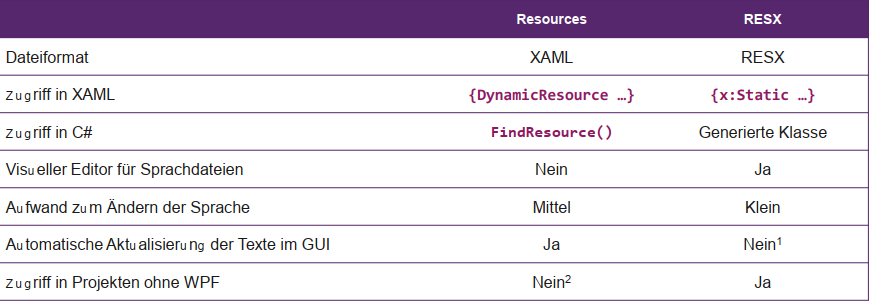
\includegraphics[scale=0.4]{images/VergleichTranslate.PNG}

\subsection{Mehrsprachigkeit – Gedanken}
Für den Zugriff im C\#-Code lohnt sich die Erstellung eines «Translation Service»\\
Dadurch bleibt der Code unabhängig von einem konkreten Übersetzungsmechanismus\\
Dies eröffnet die Möglichkeit, Übersetzungen als Properties auf dem View Model zu halten\\
Umstrittenes Thema – meine persönliche Meinung: es lohnt sich!

\subsection{Routed Events}
\textbf{UI Ereignisse, auf die reagiert werden kann}\\
• Maustaste wurde gedrückt\\
• Maus wurde bewegt\\
• Taste auf Tastatur wurde gedrückt\\
\textbf{Bewegen sich in zwei Phasen durch den Visual Tree}\\
• \textbf{Tunneling} – Abwärts bis zum fokussierten Element\\
• \textbf{Bubbeling} – Aufwärts vom fokussierten Element\\
\textbf{Bewegung kann von jedem Element gestoppt werden}\\
• Setzen von RoutedEventArgs.Handled auf \csharp{true}\\

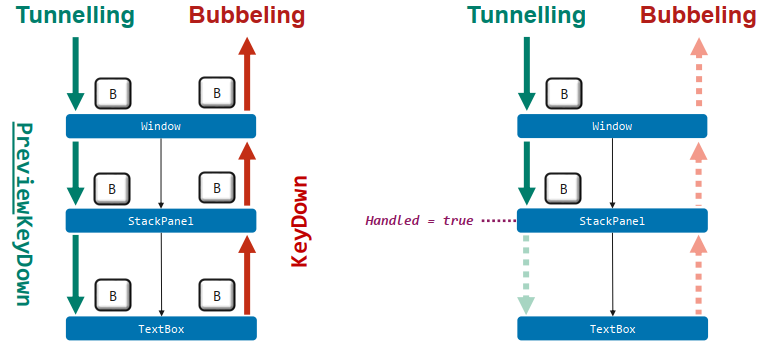
\includegraphics[scale=0.4]{images/TunnelingBubbling.PNG}

\subsection{Routed Events – Beispiel}
Möglichst wenig Logik im Code Behind\\
Bei Routed Events ist ein sparsamer und überlegter Einsatz in Ordnung\\
• Typischerweise UI-spezifische Logik\\
• Dient der Verbesserung der User Experience

\begin{minted}{xml}
<Window PreviewKeyDown="Window_OnPreviewKeyDown"
    KeyDown="Window_OnKeyDown">
    <StackPanel PreviewKeyDown="StackPanel_OnPreviewKeyDown"
                KeyDown="StackPanel_OnKeyDown">
        <TextBox PreviewKeyDown="TextBox_OnPreviewKeyDown"
                 KeyDown="TextBox_OnKeyDown" />
</StackPanel></Window>
\end{minted}
\begin{minted}{csharp}
private void Window_OnPreviewKeyDown(
object sender, KeyEventArgs e) {}
private void StackPanel_OnPreviewKeyDown(
object sender, KeyEventArgs e) {}
private void TextBox_OnPreviewKeyDown(
object sender, KeyEventArgs e) {}
\end{minted}

\section{Background Execution}
\subsection{WPF Threading Model}
In jeder WPF-Applikation gibt es mindestens zwei Threads\\
• UI Thread: Verwaltet UI, empfängt Ereignisse und führt Aktionen aus\\
• Rendering Thread: Läuft im Hintergrund, zeichnet Controls auf den Screen\\
Dadurch werden Controls auch dann neu gezeichnet, wenn der UI Thread blockiert ist\\
• Aber: der UI Thread kann keine neuen Ereignisse mehr verarbeiten\\

\subsection{Mechanismen in .NET}
NET kennt verschiedene Mechanismen für Backgrounding\\
• Klasse Task\\
• Keywords async / await\\
• Parallel LINQ (PLINQ)\\
In MGE verwenden wir die Klasse Task\\
• Einfaches Konzept\\
• Ähnlichkeit zu Runnables in Java\\
Moderne Apps verwenden async / await

\subsection{Klasse Task}
Verwendung der Klasse Task\\
• Statische Methode Task.Run(Action)\\
• Der UI Thread läuft parallel weiter\\
Nur der UI Thread darf das UI verändern\\
• Andernfalls: Exception\\
• Kennen wir aus Android\\
• Lösung in WPF: Dispatcher-Klasse\\
\csharp{Task.Run(() => {})};
\subsection{Dispatcher}
Erlaubt priorisiertes Abarbeiten von Aufgaben in einem Thread\\
Delegieren von Aufgaben an den Dispatcher\\
• Invoke() – Synchron, Aufrufer läuft erst nach Abarbeitung der Aufgabe weiter\\
• BeginInvoke() – Asynchron, Aufrufer läuft parallel zur Aufgabe weiter\\

\subsection{Zugriff auf den Dispatcher}
Fast alle WPF-Elemente erben von DispatcherObject\\
• Eigenschaft Dispatcher\\
Verwendung in WPF-Projekten\\
• Code Behind: this.Dispatcher\\
• Andere Klassen: Application.Current.Dispatcher\\
Verwendung in Nicht-WPF-Projekten\\
• Abstrahierung durch Interface nötig\\
• Implementierung des Interface im WPF-Projekt

\subsection{Auswirkungen auf View Models}
\textbf{Die gute Nachricht}\\
• Data Binding erledigt das Dispatching zum UI Thread automatisch\\
• Properties können also ohne Weiteres von einem Background Thread verändert werden\\
\textbf{Die schlechte Nachricht}\\
• ICommand.CanExecuteChanged-Events müssen manuell dispatched werden\\
• Tipp: RelayCommand entsprechend erweitern

\begin{minted}{csharp}
public sealed class RelayCommand : ICommand {
    public static Action<Action> Dispatch { get; set; }
    public void RaiseCanExecuteChanged() {
        Dispatch(() =>
            CanExecuteChanged?.Invoke(this, EventArgs.Empty));
}}
\end{minted}

\section{Xamarin}
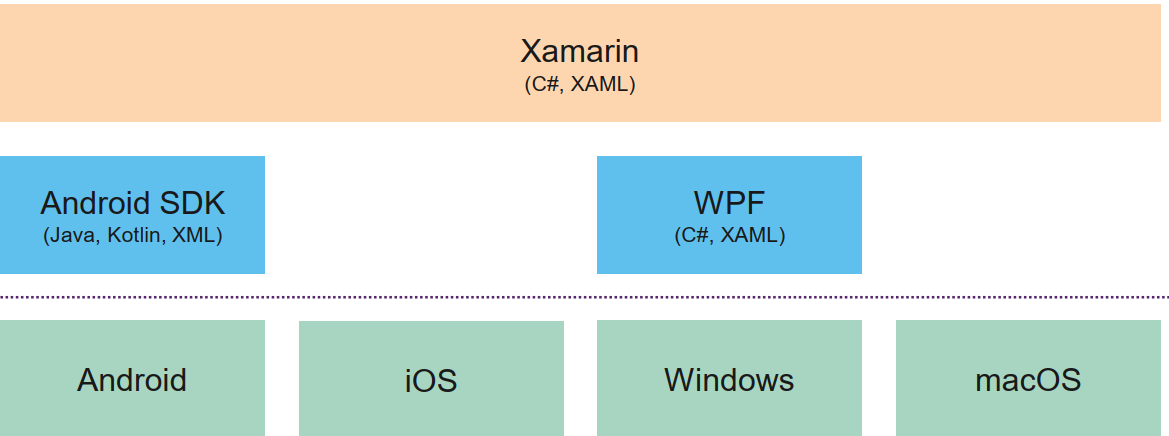
\includegraphics[scale=0.3]{images/Xamarin.PNG}
Gemeinsame Codebasis in C\# / XAML oder F\# / XAML\\
Zielplattformen: Android, iOS, iPadOS, watchOS, tvOS, macOS\\
Bei der Kompilierung werden native Apps erzeugt\\
100\%ige Verfügbarkeit der nativen APIs in C\#1\\
Benutzung gewohnter .NET-Tools (Visual Studio, NuGet, etc.)\\

Shared Code\\
• Von allen Plattformen geteilt\\
• Idealerweise möglichst gross\\
• Interfaces zur Abstraktion von Plattform Details\\
• .NET Standard Projekt\\
Platform Code\\
• Ein Projekt pro Ziel-Plattform\\
• Idealerweise möglichst klein\\
• Implementierung der Plattform-Interfaces\\
• Projekttyp abhängig von Ziel-Plattform

\subsection{Xamarin.Essentials}
Sammlung an Platform Services\\
• Sensoren Batterie, Kompass\\
• Schnittstellen Berechtigungen, Telefon\\
• Utilities Threading, Umrechnungen\\
Spart viel Zeit und Nerven\\
• Eine Schnittstelle für alle Plattformen\\
• Tipp: Trotzdem hinter Interface abstrahieren\\
Integration via NuGet

\subsection{Xamarin Traditional}
\textbf{Definition des UI pro Zielplattform}\\
• Verwendung der nativen Konzepte\\
• Android: XML, Activities, Fragmente, …\\
\textbf{Vorteile}\\
• Performance\\
• Voller Funktionsumfang der Zielplattform\\
• Portierbarkeit bestehender Apps\\
\textbf{Nachteile}\\
• Mehrfache Implementierung des UI\\
• Viele unterschiedliche Technologien

\subsubsection{Xamarin Traditional – MVVM}
\textbf{Dominierende Design Patterns}\\
• MVC in Android und iOS\\
• MVVM in .NET (XAML)\\
\textbf{Wünschenswert wäre MVVM für alles}\\
• Option 1: AndroidX (nur Android)\\
• Option 2: MvvmCross\\
\textbf{MvvmCross}\\
• Data Binding für native UIs (Beispiel Android)

\subsection{Xamarin.Forms}
\textbf{Definition des UI im Shared Code}\\
• Verwendung von XAML\\
• Tipp: eigenes Projekt für Xamarin.Forms\\
\textbf{Vorteile}\\
• UI muss nur einmalig implementiert werden\\
• Weniger Technologien\\
\textbf{Nachteile}\\
• Einschränkungen bei UI Gestaltung\\
• Leichte Einbussen bei Performance\\
• Schwierige Portierbarkeit bestehender Apps

\subsubsection{Xamarin.Forms – Renderer}
Xamarin.Forms enthält diverse Controls\\
• Beispiel: Button\\
Renderer-Klassen erledigen das Mapping von XAML-Controls auf native Controls\\
• Bestandteil von Xamarin.Forms\\
• Beispiel: ButtonRenderer für Android\\
Anpassungsmöglichkeiten\\
• Styling\\
• Eigene Renderer\\
• Eigene XAML-Controls

\subsubsection{Xamarin.Forms – Vergleich zu WPF}
Gemeinsamkeiten\\
• Aufteilung in XAML und Code Behind\\
• Application-Klasse\\
• Resources und Styles\\
• Markup Extensions\\
• Data Binding\\
• Commands\\
• Value Converter\\
\\
Unterschiede\\
• Control Libraries\\
• Anzahl UI-Projekte\\
• XAML Dialekt\\
− MainPage statt MainWindow\\
− BindingContext statt DataContext\\
− IsVisible statt Visibility\\
− Margin mit Komma statt Spaces\\
\\
Hilfsklassen in Xamarin.Forms\\
− Service Locator (Dependency Injection)\\
− Navigation Service
\subsubsection{7 Jahre Xamarin im Rückblick}
\textcolor{green}{Positive Erlebnisse}\\
• C\# und .NET
• Visual Studio auf Windows
• ReSharper
• Einfache Apps mit Xamarin.Forms
• Vielfalt an NuGet-Paketen
• Verfügbare Dokumentation
• Open Source\\
\textcolor{red}{Negative Erlebnisse}\\
• Updates
• Visual Studio auf macOS
• Native Libraries integrieren
• Komplexe Apps mit Xamarin.Forms
• Qualität der NuGet-Pakete
• Performance und Optimierungen
• Grösse der Kompilate
• Native Knowhow unerlässlich
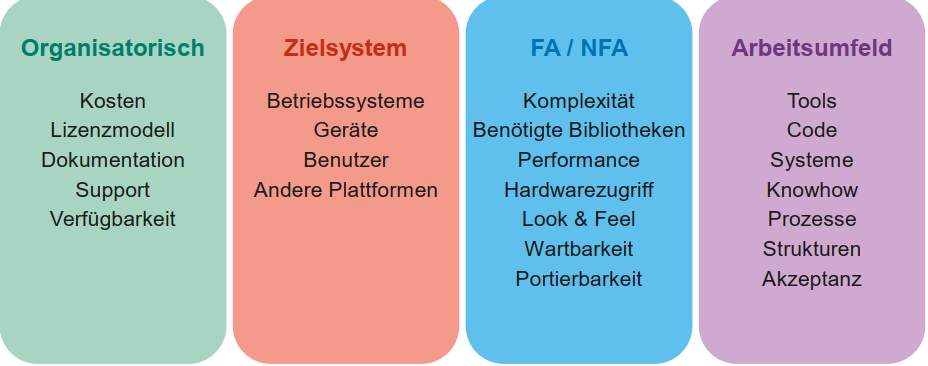
\includegraphics[scale=0.3]{images/Einflussfaktoren_Wahl.PNG}
\section{Ausblick}
\subsection{Spannende Technologien – Flutter}
Fakten\\
• Open Source SDK von Google\\
• Mobile, Desktop und Web\\
• Programmierung in Dart\\
• Eigene Rendering-Engine (Skia)\\
• Open Source bei GitHub\\
Design-Ziele\\
• Ausdrucksstarke und flexible Oberflächen\\
• Native Performance\\
• Schnelle Entwicklung

\subsection{Spannende Technologien – MAUI}
• MAUI – Multi-Platform App UI\\
• .NET UI Framework von Microsoft\\
• Framework für Mobile und Desktop\\
• Weiterentwicklung von Xamarin.Forms\\
• Basierend auf .NET 6 (ab Ende 2021)\\
• Open Source bei GitHub

\subsection{Einige Konzepte finden Sie in fast allen UI-Frameworks}
• Trennung von Layout und Logik\\
• Adaptive Layouts\\
• Main- und Background-Threads\\
• Lose Kopplung zwischen Schichten
\end{multicols*}
\end{document}